% Formelsammlung für HM1 ZHAW IT HS2020

% Dokumenteinstellungen
% ======================================================================

% Dokumentklasse (Schriftgröße 8, DIN A4, Artikel)
\documentclass[8pt,a4paper]{scrartcl}

% Zusätzliche Pakete laden
\usepackage[utf8]{inputenc}		% Zeichenkodierung: UTF-8 (für Umlaute)
\usepackage[german]{babel}		% Deutsche Sprache
\usepackage{multicol}					% Spaltenpaket
\usepackage{amsmath}				% erlaubt mathematische Formeln
\usepackage{amssymb}				% Verschiedene Symbole
\usepackage{graphicx}				% Zum Bilder einfügen benötigt

% Seitenlayout und Ränder:
\usepackage{geometry}
\geometry{a4paper,landscape, left=6mm,right=6mm, top=-1mm, bottom=5mm,includeheadfoot}
\setlength{\parindent}{0mm}

% Dokumentbeschreibung
\title{Formelsammlung Höhere Mathematik 1 ZHAW IT HS2020}
\author{Andreas Sprecher}

% Kopf- und Fußzeile
% ======================================================================
\usepackage{fancyhdr}
\pagestyle{fancy}
\fancyhf{}

\renewcommand{\headrulewidth}{0.0pt}				%obere Linie ausblenden
\renewcommand{\footrulewidth}{0.1pt}					%obere Linie ausblenden

\fancyfoot[L]{Andreas Sprecher}
\fancyfoot[C]{\textbf{Höhere Mathematik}, Seite \thepage}
\fancyfoot[R]{Stand: \todayV}

% Befehle und Befehlsüberschreibungen
% ======================================================================
\renewcommand{\familydefault}{\sfdefault}					% Schriftart SANS für bessere Lesbarkeit bei kleiner Schrift
\renewcommand{\arraystretch}{1.2}								% Array- und Tabellenabstände vergrößern
\newcommand{\todayV}{\the\day.\the\month.\the\year}	%D.M.YYYY

% Für Mengen
\newcommand{\N}{\ensuremath{\mathbb N}}
\newcommand{\R}{\ensuremath{\mathbb R}}
\newcommand{\C}{\ensuremath{\mathbb C}}

%Custom functions
\DeclareMathOperator{\arccot}{arccot}
\DeclareMathOperator{\Kern}{kern}
\DeclareMathOperator{\rang}{rang}
\DeclareMathOperator{\col}{col}
\DeclareMathOperator{\row}{row}

% Dokumentbeginn
% ======================================================================
\begin{document}

% Aufteilung in Spalten
\begin{multicols*}{3}
\setlength{\columnseprule}{0.4pt}
    \parbox{4cm}{
        \includegraphics[height=2cm]{./img/Logo.jpeg}
    }
    \parbox{4cm}{
        \emph{\Large{Höhere Mathematik 1}}
    }
    \vspace{-2mm} 

	\section{Rechnerarithmetik}
		\subsection{Maschinenzahlen}
			\begin{itemize}\itemsep0pt				
				\item $x = m \cdot B^{e}$
				\item $m: \pm 0.m_{1}...m_{n}$
				\item $B$: Basis (Binär: B=2)
				\item $e: \pm e_{1}...e_{l}$
				\item M: $\{x\epsilon R | x = \pm 0.m_{1}...m_{n}\cdot B^{\pm e_{1}...e_{l}}\} \cup \{0\}$
				\item $m_{i}, e_{i}\epsilon\{0,1,..., B-1\}$	
				\item Wert $\hat{w} = \sum m_{i}B^{\hat{e}-i}$
				\item $\hat{e} = \sum m_{i}B^{\hat{e}-i}$
			\end{itemize}
		\subsection{Approximations- und Rundungsfehler}
			\begin{itemize}\itemsep0pt	
				\item Maschinengenauigkeit eps $=\dfrac{B}{2}\cdot B^{-n}$
				\item Die Maschinengenauigkeit ist die kleinste positive Maschinenzahl, für die auf dem Rechner $1 + $eps$  \neq 1$ gilt.
			\end{itemize}		
		
			\subsubsection{Konditionierung}
    				\begin{itemize}\itemsep0pt			
    					\item Konditionszahl $K:= \dfrac{|f'(x)|\cdot |x|}{|f(x)|} $
    					\item Näherungsweise Angabe, um wieviel sich der relative Fehler von x vergrössert bei einer Funktionsauswertung f(x).
    					\item Ein Problem ist gut konditionierte, wenn die Konditionszahl klein ist.

				\end{itemize}		
		
    			\subsubsection{Absoluter Fehler}
    				\begin{itemize}\itemsep0pt			
    					\item $|\tilde{x} - x|$	
					\item $|f(\tilde{x})-f(x)|\approx |f'(x)|\cdot |\tilde{x} - x|$
				\end{itemize}
			\subsubsection{Relativer Fehler}	
				\begin{itemize}\itemsep0pt	
					\item $\dfrac{|\tilde{x} - x|}{|x|}$
					\item $\dfrac{|f(\tilde{x})-f(x)|}{|f(x)|}\approx \dfrac{|f'(x)|\cdot |x|}{|f(x)|} \cdot \dfrac{|\tilde{x} - x|}{|x|}$
				\end{itemize}
   
	\section{Nullstellenproblemen}
		\subsection{Fixpunktgleichung}
			\begin{itemize}\itemsep0pt	
				\item Idee: $f(x) = F(x) - x$
				\item $F(x) = x$
			\end{itemize}
		\subsection{Fixpunktiteration}
			\begin{itemize}\itemsep0pt	
				\item $x_{n+1} \equiv F(x_{n})$
			\end{itemize}
			\subsubsection{Anziehender Fixpunkt}
				\begin{itemize}\itemsep0pt	
					\item Ist $|F'(x)| < 1$, so konvergiert $x_{n}$ gegen $\bar{x}$, falls der Startwert $x_{0}$ nahe genug bei $\bar{x}$ liegt.
				\end{itemize}
			\subsubsection{Abstossender Fixpunkt}
			\begin{itemize}\itemsep0pt	
					\item Ist $|F'(x)| > 1$, so konvergiert $x_{n}$ für keinen Startwert $x_{0}\neq \bar{x}$.
			\end{itemize}

		\subsection{Banachsche Fixpunktsatz}
			Wenn eine Lipschnitz-Konstante $\alpha$ mit:
			
			\begin{itemize}\itemsep0pt	
				\item $F: [a,b] \rightarrow [a,b]$
				\item $0<\alpha <1$
				\item $|F(x) - F(y)| \leq \alpha |x-y|$ mit $x,y \epsilon [a,b]$
			\end{itemize}
			
			 existiert, dann gilt:
			 
			 \begin{itemize}\itemsep0pt	
				\item F hat genau einen Fixpunkt $\bar{x}$ in $[a,b]$
				\item Die Fixpunktiteration $x_{n+1} = F(x_{n})$ konvergiert gegen $\bar{x}$ für alle Startwerte $x_{0} \epsilon [a,b]$
				\item a-priori Abschätzung $|x_{n} - \bar{x}| \leq \dfrac{\alpha^{n}}{1-\alpha}\cdot |x_{1}-x_{0}|$ 
				\item a-posteriori Abschätzung $|x_{n} - \bar{x}| \leq \dfrac{\alpha}{1-\alpha}\cdot |x_{n}-x_{n-1}|$ 
			\end{itemize}
			 
			 
		\subsection{Newtonverfahren}
			\begin{itemize}\itemsep0pt	
				\item $x_{n+1} = x_{n} - \dfrac{f(x_{n})}{f'(x_{n})}$
			\end{itemize}
			\subsubsection{Vereinfachte Newtonverfahren}
				\begin{itemize}\itemsep0pt	
					\item $x_{n+1} = x_{n} - \dfrac{f(x_{n})}{f'(x_{0})}$
				\end{itemize}
		\subsection{Sekantenverfahren}
			\begin{itemize}\itemsep0pt	
				\item $x_{n+1} = x_{n} - \dfrac{x_{n - x_{n-1}}}{f(x_{n}) - f(x_{n-1})} \cdot f(x_{n})$
			\end{itemize}
		\subsection{Konvergenzordnung $q$}
			\begin{itemize}\itemsep0pt	
				\item $|x_{n+1} - \bar{x}| \leq c \cdot |x_{n} - \bar{x}|^{q}$				
				\item $c>0$
				\item $q\geq 1$
				\item Für $q=1$ muss $c<1$ gelten
			\end{itemize}
		
		
			Für einfache Nullstellen konvergiert:
			\begin{itemize}\itemsep0pt	
				\item Das Newton-Verfahren quadratisch (q=2)
				\item Das vereinfachte Newton-Verfahren linear (q=1)
				\item Das Sekantenverfahren $q = \dfrac{1+\sqrt{5}}{2} \approx 1.618$
			\end{itemize}
		
		
	\section{Lineare Gleichungssysteme}
		\subsection{Dreiecksmatrix}
			\begin{itemize}\itemsep0pt		
				\item Untere Dreiecksmatrix: $\begin{pmatrix}2&0&0\\1&2&0\\1&2&1\end{pmatrix}$
				\item Obere normierte Dreiecksmatrix: $\begin{pmatrix}1&2&1\\0&1&2\\0&0&1\end{pmatrix}$
			\end{itemize}
			
		\subsection{Gauss-Algorithmus}
			\begin{itemize}\itemsep0pt		
				\item Ausgangslage: $Ax = b$
				\item $\begin{pmatrix}a_{11}&a_{12} | b_{1}\\a_{21}&a_{22}|b_{2}\end{pmatrix} = $ \\ $\begin{pmatrix}a_{11}&a_{12} | b_{1}\\0&a_{22}-a_{12}\cdot \dfrac{a_{21}}{a_{11}}|b_{2}-b_{1}\cdot \dfrac{a_{21}}{a_{11}}\end{pmatrix} $
			\end{itemize}
			\subsubsection{Spaltenpivotisierung}
			$\begin{pmatrix}1&1&1\\2&1&1\\1&2&2\end{pmatrix} \rightarrow \begin{pmatrix}2&1&1\\1&1&1\\1&2&2\end{pmatrix} \rightarrow \begin{pmatrix}2&1&1\\1&2&2\\1&1&1\end{pmatrix}$
	
		\subsection{LR-Zerlegung}	
			\begin{itemize}\itemsep0pt				
				\item $A = L \cdot R$
				\item $L$ ist eine untere normierte Dreiecksmatrix
				\item $R$ ist eine obere Dreiecksmatrix $r_{ii} \neq 0$
				\item $A=\begin{pmatrix}1&1&2\\2&1&1\\1&2&2\end{pmatrix}$
				\item  $A^{*}=\begin{pmatrix}2&1&1\\1&1&2\\1&2&2\end{pmatrix}$, $P_{1}=\begin{pmatrix}0&1&0\\1&0&0\\0&0&1\end{pmatrix}$
				\item $A_{1}^{*}=\begin{pmatrix}2&1&1\\0&0.5&1.5\\0&1.5&1.5\end{pmatrix}$, $L=\begin{pmatrix}1&0&0\\0.5&1&0\\0.5&?&1\end{pmatrix}$
				\item $A_{1}^{**}=\begin{pmatrix}2&1&1\\0&1.5&1.5\\0&0.5&1.5\end{pmatrix}$, $P_{2}=\begin{pmatrix}1&0&0\\0&0&1\\0&1&0\end{pmatrix}$
				\item $R=\begin{pmatrix}2&1&1\\0&1.5&1.5\\0&0&1\end{pmatrix}$, $L=\begin{pmatrix}1&0&0\\0.5&1&0\\0.5&0.33&1\end{pmatrix}$
				\item 	$P = P_{2} \cdot P_{1} = \begin{pmatrix}0&1&0\\0&0&1\\1&0&0\end{pmatrix}$
				\item $Ly = Pb$
				\item $Rx = y$
			\end{itemize}
			
		\subsection{QR-Zerlegung}	
			\begin{itemize}\itemsep0pt				
				\item $Q^{T}\cdot Q =I \rightarrow Q$ ist orthogonal 
				\item 	orthogonal $\rightarrow Q^{-1} = Q^{T} \rightarrow Q$ ist regulär
				\item 	$Q^{T} = Q \rightarrow Q$ ist symmetrisch 
			\end{itemize}
		
			\subsubsection{Householder-Matrizen}
				\begin{itemize}\itemsep0pt				
					\item $u$ normierter Vektor (Länge 1)
					\item $H := I - 2uu^{T}$
					\item $H$ ist symmetrisch und orthogonal
					\item $v_{1} := a_{1} + $ sign$(a_{11}) \cdot |a_{1}| \cdot e_{1}$
					\item $u_{1} := \dfrac{1}{|v_{1}|}v_{1}$
					
				
				\end{itemize}
				
			\subsubsection{Vorgehen}
				\begin{itemize}\itemsep0pt	
					\item $A=\begin{pmatrix}1&1&2\\2&1&1\\1&2&2\end{pmatrix}$, $a_{1}=\begin{pmatrix}1\\2\\1\end{pmatrix}$, $e_{1}=\begin{pmatrix}1\\0\\0\end{pmatrix}$
					\item $v_{1} = \begin{pmatrix}3.45\\2\\1\end{pmatrix}$, $u_{1} = \begin{pmatrix}0.84\\0.49\\0.24\end{pmatrix}$
					\item $H_{1} = Q_{1} = \begin{pmatrix}-0.41&-0.82&-0.41\\-0.82&0.53&-0.24\\-0.41&-0.24&0.88\end{pmatrix}$
					\item $Q_{1}A= \begin{pmatrix}-2.45&-2.04&-2.45\\0&-0.76&-1.58\\0&1.12&0.71\end{pmatrix}$
					\item $ A_{2} = \begin{pmatrix}-0.76&-1.58\\1.12&0.71\end{pmatrix}$
					\item $v_{2} = \begin{pmatrix}-2.12\\1.12\end{pmatrix}$, $u_{2} = \begin{pmatrix}-0.88\\0.47\end{pmatrix}$
					\item $H_{2} = \begin{pmatrix}-0.56&0.83\\0.83&0.56\end{pmatrix}$
					\item $Q_{2} = \begin{pmatrix}1&0&0\\0&-0.56&0.83\\0&0.83&0.56\end{pmatrix}$
					\item $Q= Q_{1}^{T} Q_{2}^{T}$
					\item $R= Q_{1}Q_{2}A$
					
				\end{itemize}
		
		\subsection{Fehlerrechnung}
			\begin{itemize}\itemsep0pt	
				\item Ziel: Von Residuum auf Fehler von x schliessen.
				\item $A \tilde{x} = \tilde{b }= b + \Delta b$
				\item Residuum: $\Delta b$
				\item Fehler von x: $\Delta x = \tilde{x}-x$
			\end{itemize}
		
		
			\subsection{Vektornormen / Matrixnormen}
				\subsubsection{1-Norm}			
					\begin{itemize}\itemsep0pt	
						\item $||\begin{pmatrix}-1\\2\\3\end{pmatrix}||_{1} = 1+2+3=6$
						\item $||\begin{pmatrix}1&2&3\\3&4&-2\\7&-3&5\end{pmatrix}||_{1} = $ max(1+3+7, 2+4+3, 3+2+5) = 11
					\end{itemize}
				\subsubsection{2-Norm}			
					\begin{itemize}\itemsep0pt	
						\item $||\begin{pmatrix}-1\\2\\3\end{pmatrix}||_{2} = \sqrt{1^{2}+2^{2}+3^{2}}=\sqrt{14}$
					\end{itemize}
				\subsubsection{$\infty-$Norm}			
					\begin{itemize}\itemsep0pt	
						\item $||\begin{pmatrix}-1\\2\\3\end{pmatrix}||_{\infty} = $max$(1+2+3)=3$
						\item $||\begin{pmatrix}1&2&3\\3&4&-2\\7&-3&5\end{pmatrix}||_{\infty} = $ max(1+2+3, 3+4+2, 7+3+5)=15
					\end{itemize}
			
			\subsection{Abschätzung für fehlerbehaftete Vektoren}
				\begin{itemize}\itemsep0pt	
					\item $||x-\tilde{x}|| \leq ||A^{-1}||\cdot ||b-\tilde{b}||$
					\item $\dfrac{||x-\tilde{x}||}{||x||} \leq ||A||\cdot ||A^{-1}||\cdot \dfrac{||b-\tilde{b}||}{||b||}$, falls $||b||\neq0$
					\item Konditionszahl cond$(A) = ||A||\cdot ||A^{-1}||$
				\end{itemize}

			\subsection{Abschätzung für fehlerbehaftete Matrix}
				\begin{itemize}\itemsep0pt	
					\item $\tilde{A} \cdot \tilde{x} = \tilde{b}$
					\item Wenn: cond$(A)\cdot \dfrac{||A-\tilde{A}||}{||A||} < 1$
					\item Dann: $\dfrac{||x-\tilde{x}||}{||x||} \leq \dfrac{cond(A)}{1-cond(A)\cdot \dfrac{||A-\tilde{A}||}{||A||}}\cdot (\dfrac{||A-\tilde{A}||}{||A||} + \dfrac{||b-\tilde{b}||}{||b||} ) $
				\end{itemize}
				
			\subsection{Iterative Verfahren}
				\begin{itemize}\itemsep0pt	
					\item Ein Startvektor $x^{(0)}$ wird solange iteriert ($x^{(k+1)} = F(x^{(k)})$), bis x gegen das Gleichungssystem $Ax = b$ konvergiert
					\item Ein hochgestellter Index in Klammern $x^{(k)}$ bezeichnet einen Vektor aus $R^{n}$ nach der k-ten Iteration
					\item A = L + D + R
					\item $A = \begin{pmatrix}0&0&0\\a_{21}&0&0\\a_{31}&a_{32}&0\end{pmatrix} + \begin{pmatrix}a_{11}&0&0\\0&a_{22}&0\\0&0&a_{33}\end{pmatrix} + \begin{pmatrix}0&a_{12}&a_{13}\\0&0&a_{23}\\0&0&0\end{pmatrix}$
					\item Matrizen L und R entsprechen nicht den Matrizen der LR-Zerlegung
				\end{itemize}


			\subsection{Das Jacobi-Verfahren / Gesamtschrittverfahren}
				\begin{itemize}\itemsep0pt	
					\item $Dx^{(x+1)} = -(L+R)x^{(k)} + b$
					\item $x^{(x+1)} = -D^{-1}(L+R)x^{(k)} + D^{-1}b$
					\item $B = -D^{-1}(L+R)$
				\end{itemize}
			
			\subsection{Das Gauss-Seidel-Verfahren / Einzelschrittverfahren}
				\begin{itemize}\itemsep0pt	
					\item $(D+L)x^{(x+1)} = -Rx^{(k)} + b$
					\item $x^{(x+1)} = -(D+L)^{-1}Rx^{(k)} + (D+L)^{-1}b$
					\item $B = -(D+L)^{-1}R$
				\end{itemize}
		
			\subsection{Konvergenz}
				\begin{itemize}\itemsep0pt	
					\item Falls A diagonaldominant ist, konvergiert das Gesamtschrittverfahren und das Einzelschrittverfahren für Ax = b	
					\item Es gibt nicht diagonaldominante Matrizen, für die die Verfahren trotzdem konvergieren kann
					\item Ein notwendiges und hinreichendes Kriterium ist, dass der Spektralradius $\rho(B) < 1$
				\end{itemize}			
			
				\subsubsection{Anziehender oder abstossender Fixpunkt}
					\begin{itemize}\itemsep0pt	
						\item $x^{(n+1)} = Bx^{(n)} + b$
						\item $\bar{x}$ anziehender Fixpunkt, wenn $||B||<1$
						\item $\bar{x}$ abstossender Fixpunkt, wenn $||B||>1$
					\end{itemize}
					
				\subsubsection{Abschätzung}
					\begin{itemize}\itemsep0pt	
						\item $x^{(n+1)} = Bx^{(n)} + b$
						\item a-priori Abschätzung: $||x^{(n)} - \bar{x}|| \leq \dfrac{||B||^{n}}{1-||B||}\cdot ||x^{(1)}-x^{(0)}||$ 
						\item a-posteriori Abschätzung: $||x^{(n)} - \bar{x}|| \leq \dfrac{||B||}{1-||B||}\cdot ||x^{(n)}-x^{(n-1)}||$ 
					\end{itemize}
					
				\subsubsection{Diagonaldominanz}
					\begin{itemize}\itemsep0pt	
						\item A ist diagonaldominant, wenn das Zeilensummenkriterium oder das Spaltensummenkriterium gilt
						\item Zeilensummenkriterium: für alle i = 1,...,n: $|a_{ii}| > \sum_{j=1, j \neq i}^{n}|a_{ij}|$
						\item Spaltensummenkriterium: für alle j = 1,...,n: $|a_{jj}| > \sum_{i=1, i \neq j}^{n}|a_{ij}|$
					\end{itemize}
				
				
		
		\subsection{Komplexe Zahlen}
			\begin{itemize}\itemsep0pt	
				\item Eine komplexe Zahl $z$ ist ein geordnetes Paar $(x, y)$ zweier reeller Zahlen $x$ und $y$
				\item $z = x + iy$
				\item $z^{*} = x - iy$
				\item $|z|= \sqrt{x^{2}+y^{2}}$
				\item $i^{2} = -1$
				\item Realteil von $z: Re(z) = x$
				\item Imaginärteil von $z: Im(z) = y$
			\end{itemize}
			
			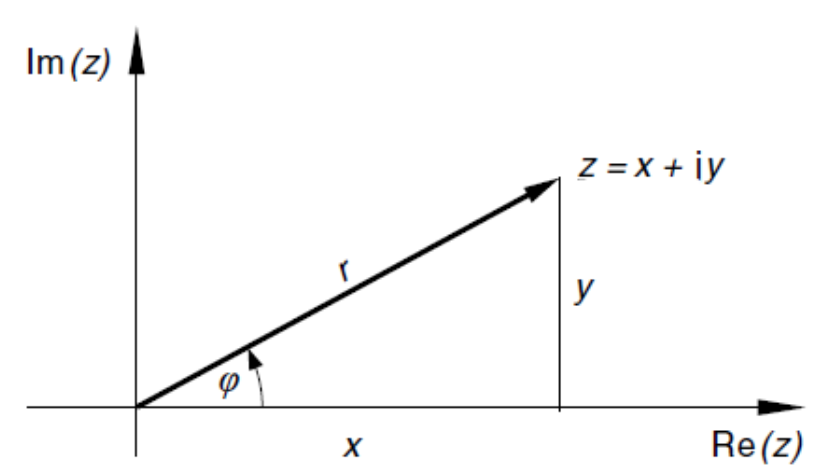
\includegraphics[height=5cm]{./img/komplex.png}
			
			\begin{itemize}\itemsep0pt	
				\item Normalform: $z = x + iy$
				\item Trigonometrische Form: $z = r(cos(\varphi)+i\cdot sin(\varphi))$
				\item Exponentialform: $z = re^{i\varphi}$
			\end{itemize}
			
			\subsubsection{Rechenregeln}
				\begin{itemize}\itemsep0pt	
					\item Addition: $z_{1} + z_{2} = (x_{1} + x_{2})+i(y_{1} + y_{2})$
					\item Subtraktion: $z_{1} - z_{2} = (x_{1} - x_{2})+i(y_{1} - y_{2})$
					\item Multiplikation: $z_{1} \cdot z_{2} = (x_{1}x_{2} - y_{1}y_{2}) - i(x_{1}y_{2} + x_{2}y_{1})$
					\item$z_{1} \cdot z_{2} =  r_{1}e^{i\varphi_{1}} \cdot  r_{2}e^{i\varphi_{2}} =  r_{1}r_{2}e^{i(\varphi_{1}+\varphi_{2})}$
					\item Division: $\dfrac{z_{1}}{z_{2}} = \dfrac{z_{1} \cdot z_{2}^{*} }{z_{2} \cdot z_{2}^{*} }$
					\item$\dfrac{z_{1}}{z_{2}} = \dfrac{r_{1}e^{i\varphi_{1}}}{r_{2}e^{i\varphi_{2}}} = \dfrac{r_{1}}{r_{2}}e^{i(\varphi_{1} - \varphi_{2})}$
				\end{itemize}
				
				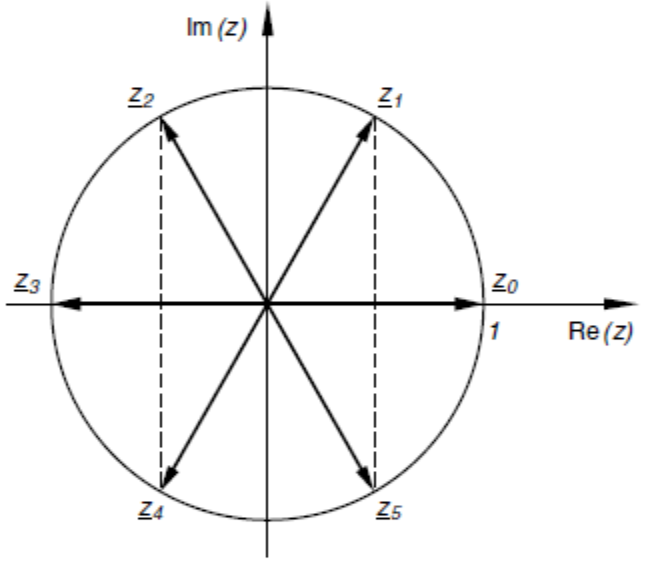
\includegraphics[height=6cm]{./img/komplex2.png}
				\begin{itemize}\itemsep0pt	
					\item Die Lösungen der Gleichung $z^{6} = 1$
				\end{itemize}
										
			\subsection{Eigenwerte und Eigenvektoren}	
				\begin{itemize}\itemsep0pt				
					\item $Ax = \lambda x$
					\item Eigenwert $\lambda$
					\item Eigenvektor $x$
					\item Der Nullvektor wird als triviale Lösung nicht berücksichtigt
					\item Eigenvektoren werden i.d.R. auf die Länge 1 normiert
					\item $(A - \lambda I_{n})x = 0$
				\end{itemize}
			
			\subsubsection{Charakteristisches Polynom / Spur}
  			Spur von A $= tr(A)=a_{11} +a_{22} +...+a_{nn} =\lambda_{1} +\lambda_{2} +...+\lambda_{n}$

			\subsubsection{Algebraische Vielfachheit / Spektrum}
				\begin{itemize}\itemsep0pt		
					\item Das Spektrum $\sigma(A)$ ist die Menge aller Eigenwerte von A
					\item $(1-\lambda)^{2} = 0$ \qquad Algebraische Vielfachheit = 2
					\item $\lambda = 0$ \qquad \qquad \qquad Algebraische Vielfachheit = 1
				\end{itemize}
				
			\subsubsection{Eigenraum}				
				\begin{itemize}\itemsep0pt		
					\item Die Eigenvektoren zum Eigenwert $\lambda$ bilden zusammen mit dem Nullvektor 0 einen Unterraum
					\item Der Eigenraum des Eigenwertes $\lambda$ ist die Lösungsmenge des homogenen lin. Gleichungssystems $(A - \lambda I_{n})x = 0$
					\item Weist nur dann eine nicht-triviale Lösung auf, wenn gilt: $Rg(A - \lambda I_{n}) < n$
					\item \textbf{Geometrische Vielfachheit}: $n - Rg(A - \lambda I_{n})$
				\end{itemize}
			
			\subsubsection{Vielfachheit}		
				\begin{itemize}\itemsep0pt	
					\item Geometrische und algebraische Vielfachheit eines Eigenwerts müssen nicht gleich sein
					\item Die geom. Vielfachheit ist aber stets kleiner oder gleich der algebraischen Vielfachheit
				\end{itemize}
				
			\subsubsection{Ähnliche Matrizen / Diagonalisierbarkeit}
				\begin{itemize}\itemsep0pt	
					\item A und B sind ähnlich: $B = T^{-1}1AT$
					\item Ist B eine Diagobalmatrix ist A \textbf{diagonalisierbar}
					\item Ähnliche Matrizen haben dieselben Eigenwerte, inkl. deren algebraischer Vielfachheit.
					\item Ist x ein Eigenvektor zum Eigenwert $\lambda$ von B, dann ist Tx ein Eigenvektor zum Eigenwert $\lambda$ von A
					\item In einer diagonalisierbar Matrix sind die n Diagonalelemente von D die Eigenwerte von A
					\item In einer diagonalisierbar Matrix stehen die n linear unabhängigen Eigenvektoren von A in den Spalten von T
				\end{itemize}
				
			\subsubsection{Determinante von $A\in \mathbb K^{n\times n}$: $\det(A)=|A|$}

				\begin{itemize}\itemsep0pt
				\item $A=\begin{pmatrix}2&2&2\\1&2&1\\1&2&1\end{pmatrix},|A_{12}| = \begin{pmatrix}a_{21}&a_{23}\\a_{31}&a_{33}\end{pmatrix},\begin{pmatrix}1&1\\1&1\end{pmatrix} $ 
					\item $|A|=\sum\limits_{i=1}^n (-1)^{i+j} \cdot a_{ij} \cdot |A_{ij}|$ \qquad Entwicklung n. $j$-ter Spalte
					\item $|A|=\sum\limits_{j=1}^n (-1)^{i+j} \cdot a_{ij} \cdot |A_{ij}|$ \qquad Entwicklung n. $i$-ter Zeile
					\item $\det\begin{pmatrix}A&0\\C&D\end{pmatrix}=\det\begin{pmatrix}A&B\\0&D\end{pmatrix}=\det(A)\cdot\det(D)$
					\item $\begin{vmatrix}\lambda_1&&* \\ &\ddots& \\ 0&&\lambda_n \end{vmatrix} = \lambda_1\cdot \ldots\cdot \lambda_n = \begin{vmatrix} \lambda_1&&0  \\  &\ddots& \\  *&&\lambda_n \end{vmatrix}$
					\item $A=B \cdot C \quad \Rightarrow \quad |A|=|B| \cdot |C|$
					\item $\det(A)=\det(A^\top)$
					\item Hat $A$ zwei gleiche Zeilen/Spalten $\Rightarrow |A|=0$
					\item $\det(\lambda A)=\lambda^n \det(A)$
					\item Ist $A$ invertierbar, so gilt: $\det(A^{-1})=(\det(A))^{-1}$
					\item $\det(AB) = \det(A) \det(B) = \det(B) \det(A) = \det(BA)$
				\end{itemize}
				\textbf{Umformung Determinante}
				\begin{itemize}\itemsep0pt
					\item Vertauschen von Zeilen/Spalten ändert Vorzeichen von $|A|$
					\item Zeile/Spalte mit $\lambda$ multiplizieren, $|A|$ um Faktor $\lambda$ größer
					\item Addition des $\lambda$-fachen der Zeile X zur Zeile Y ändert $|A|$ nicht 
				\end{itemize}
				\textbf{Vereinfachung für Spezialfall $A\in \mathbb K^{2\times 2}$}\\
				$A=\begin{pmatrix}a&b\\c&d\end{pmatrix} \Rightarrow \det(A)=|A|=ad-bc$

			\subsubsection{Äquivalente Aussagen für $A\in \mathbb K^{n\times n}$}
				\begin{tabular}{ll}
					1)  $A$ ist invertierbar & 2) $\dim(\col(A))=\dim(\row(A))=n$\\
					3)  $\Kern(A)={0}$ & 4) Die strenge ZSF von $A$ ist $\mathbb{I}_n$\\
					5) $\det(A)\ne0$ & 6) Zeilen/Spalten von $A$ linear unabhängig\\
					7) $Ax=b$ hat eine & 8) 0 ist kein Singulärwert von $A$\\\ \ \ \ eind. Lös. $\forall b\in\mathbb{R}^n$ & 9) Lineare Abbildung ist bijektiv\\
					10)  $\rang(A)=n$ & 11) 0 ist kein Eigenwert von $A$\\

				\end{tabular}			
			
			

    


\end{multicols*}

% Dokumentende % ======================================================================
\end{document}
